%! Boxplots, Outliers, and Resistance — Unit 2, Lesson 2.3 — Guided Notes & Practice
% THE in-class document, in the MAIN IDEAS / NOTES shape (LESSON_SHAPE.md §1): the vocabulary
% box, the hook, then ONE two-column guidednotes table. Each row is one idea — a label on the
% left; on the right one or two COMPLETE printed sentences, ONE large pre-drawn display the
% student reads or names, then a bold prompt and a two-across grid of numbered problems.
% Problems run 1..22. Unit 2 timing (5 / 45 / 5 / 5): I do ~25 min (rows 1-4), Guided
% Practice ~20 min (row 5). 4-5 pages at 12pt.
% DENSITY: no \blank{} in this component — every answer is written in a problem's own space
% or in a \labelbox on a display; every display is pre-drawn (TikZ) and read. Problem 4 asks
% students to FINISH a boxplot on a provided, pre-scaled axis (completing marks, not a sketch).
%   I DO   : the teacher reads the definition, marks up the display, works the first problem
%            of each grid (1, 5, 9, 13).
%   WE DO  : the class works the rest of each grid, students holding the pen; the last row,
%            Guided Practice (19-22), is worked entirely together on the Maple Grove shelter.
%   YOU DO : nothing on this page — ../homework/ IS the individual practice, assigned at
%            Close & Assign and done outside class.
% THE TRAP is problem 7 (a 16-minute delivery that LOOKS far but sits inside the lower fence).
% THE CRUX is problem 17 (row 4, "Resistance"): the hook vote re-taken — removing the 55 drops
% the mean 3 minutes and the median half a minute (PS.DS.2d). Problem 21 is the crux
% transferred to the shelter; problem 22 is the report choice (median/IQR for outlier data).
%
% THE DATA (all checked by hand; quartiles = medians of the lower and upper halves, the overall
% median left OUT of both halves when n is odd; SD = SAMPLE standard deviation, divide by n-1)
%   Pine Street Pizza, ten Friday deliveries (min): 20 22 23 24 25 26 27 28 30 55
%     sum 280, mean 28; median (25+26)/2 = 25.5; Q1 = med(20,22,23,24,25) = 23;
%     Q3 = med(26,27,28,30,55) = 28; IQR 5; step 7.5; fences 15.5 and 35.5; 55 the only
%     outlier; modified whisker stops at 30. s = sqrt(888/9) = 9.93 -> 9.9.
%   Without the 55 (nine): sum 225, mean 25; median 25; Q1 = med(20,22,23,24) = 22.5;
%     Q3 = med(26,27,28,30) = 27.5; IQR 5. s = sqrt(78/8) = 3.12 -> 3.1.
%   Trap (problem 7): min 16 instead of 20 -> Q1 = med(16,22,23,24,25) = 23 unchanged;
%     16 > 15.5, NOT an outlier.
%   Saturday summary (problem 4): 18, 22, 24, 27, 33.
%   Week's 40 deliveries (ogive): cumulative % at 15,20,25,30,35,40,45 min =
%     0, 25, 50, 75, 90, 95, 100 -> Q1 20, median 25, Q3 30, IQR 10; 35 min = 90th
%     percentile; 10% of 40 = 4 free deliveries; 30 min = 75th percentile.
%   Guided Practice, Maple Grove shelter, ten dogs (days): 2 4 4 5 6 7 10 10 15 37
%     sum 100, mean 10; median (6+7)/2 = 6.5; Q1 = med(2,4,4,5,6) = 4; Q3 = med(7,10,10,15,37)
%     = 10; IQR 6; step 9; fences -5 and 19; 37 the only outlier; whisker stops at 15.
%     Without the 37: sum 63, mean 7; median 6; Q1 = 4; Q3 = 10; IQR 6.
%     s = sqrt(940/9) = 10.2 with, sqrt(130/8) = 4.0 without (plan only).
%
% PAGE LOCKSTEP with notes_key/: the key differs ONLY in saar-key for saar-boxes, the header's
% "--- Answer Key", \vterm -> \vtermans, the hook's two \writeline -> \ansline, and the answer
% argument of every \pcell, \writespace and \labelbox. KEEP EVERY \pcell ON ONE SOURCE LINE.
% TABLE MECHANICS: inside a cell, `\\` ENDS THE ROW — break lines with \par. A row cannot break
% across pages: the figure gets its own sub-row (`\\` then `& ...`) and EACH GRID ROW is its own
% sub-row — close the probgrid, `\\ &`, reopen as probgrid* (no top rule).
\documentclass[12pt]{article}
\usepackage{saar-article}
\usepackage{saar-boxes}
\newcommand{\TallMath}[1]{$\displaystyle #1\rule[-1.4em]{0pt}{3.2em}$}
% Vocabulary rows: a FIXED-HEIGHT row carrying the term label and OPEN writing space — no
% underline beside the term and no rule line (user correction 2026-09-06). The key fills
% exactly the same height, so the box cannot drift blank vs. keyed. Copied from
% unit01/lesson02/notes/main.tex; keep key definitions to two lines.
\newcommand{\termrowheight}{2.3cm}
\newlength{\termrowinset}\setlength{\termrowinset}{7pt}
\newcommand{\vterm}[1]{%
  \par\noindent\begin{minipage}[t][\termrowheight][t]{\linewidth}%
    \vspace*{\termrowinset}%
    \textbf{\textcolor{cerulean}{#1:}}%
  \end{minipage}\par}
\newcommand{\vtermans}[2]{%
  \par\noindent\begin{minipage}[t][\termrowheight][t]{\linewidth}%
    \vspace*{\termrowinset}%
    \textbf{\textcolor{cerulean}{#1:}}\quad\ans{#2}%
  \end{minipage}\par}

\begin{document}

\pageheader{Unit 2, Lesson 2.3}{Guided Notes \& Practice}
% NAMESTRIP: no \namedateperiod here. The student writes their name once, on the
% cover this component is stapled behind.

\vspace{0.15in}

\boxguard[16]
\begin{vocabbox}
\small
Fill in each term \textbf{as we name it} in the notes below.
\vterm{Boxplot}
\vterm{Outlier}
\vterm{Modified boxplot}
\vterm{Cumulative relative frequency graph}
\vterm{Resistant}
\end{vocabbox}

\boxguard[12]
\begin{hookbox}
\small
Pine Street Pizza timed its ten Friday-night deliveries, in minutes: $20, 22, 23, 24, 25, 26,
27, 28, 30, 55$. The $55$ was the night the driver got a flat tire, and the manager wants to
throw it out.

\vspace{3pt}
\textbf{Which number drops more when the $55$ is removed?} Circle one: \quad the mean \qquad
the median \qquad they drop about the same \quad --- and say why. We vote again at problem~17.
\par\writeline
\par\writeline
\end{hookbox}

\small
\begin{guidednotes}
% ── ROW 1: five numbers, one picture ─────────────────────────────────────────
\mainidea[Five numbers, one picture]{Boxplot} &
A \textbf{boxplot} draws the five-number summary --- minimum, $Q_1$, median, $Q_3$, maximum
--- on a number line: a box from $Q_1$ to $Q_3$ with a line at the median, and a whisker out to
each extreme. ($Q_1$ and $Q_3$ are the medians of the lower and upper halves; when the count is
odd, leave the median out of both halves.) \textbf{The four sections have different lengths,
but each holds about the same number of values.}
\\
& {\centering
\begin{tikzpicture}[x=0.24cm, y=1cm]
  \node[anchor=south west, font=\scriptsize\bfseries\color{cerulean}] at (14,1.5)
    {Pine Street Pizza --- ten Friday deliveries};
  \draw[->, thick] (14,0) -- (61,0);
  \foreach \x in {15,...,60} { \draw (\x,0.04) -- (\x,-0.04); }
  \foreach \x in {15,20,...,60} {
    \draw (\x,0.09) -- (\x,-0.09); \node[below, font=\scriptsize] at (\x,-0.09) {\x}; }
  \node[font=\scriptsize, anchor=north] at (37.5,-0.45) {delivery time (minutes)};
  \draw[thick, cerulean] (20,0.9) -- (23,0.9);
  \draw[thick, cerulean] (28,0.9) -- (55,0.9);
  \draw[thick, cerulean] (20,0.7) -- (20,1.1);
  \draw[thick, cerulean] (55,0.7) -- (55,1.1);
  \draw[thick, cerulean, fill=frost] (23,0.55) rectangle (28,1.25);
  \draw[very thick, cerulean] (25.5,0.55) -- (25.5,1.25);
\end{tikzpicture}\par\vspace{5pt}
Each of the four sections holds about \labelbox{1.3cm}{} of the deliveries, so the box holds
the middle \labelbox{1.3cm}{}\par}
\\
& \notesprompt{Read it, then build one.}
\begin{probgrid}{|Y|Y|}
\pcell{1}{Read Friday's five-number summary off the boxplot.}{1.3cm}{} & \pcell{2}{The right whisker is nine times as long as the left one. Does it hold nine times as many deliveries? Explain.}{2.0cm}{} \\ \hline
\end{probgrid}
\\
& \begin{probgrid}*{|Y|Y|}
\pcell{3}{About what percent of Friday's deliveries took $28$ minutes or less? Say it in context.}{1.7cm}{} & \pcell{4}{Saturday: min $18$, $Q_1 = 22$, median $24$, $Q_3 = 27$, max $33$. Finish its boxplot on this axis.\par\smallskip{\centering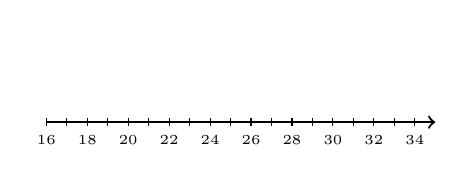
\begin{tikzpicture}[x=0.26cm, y=1cm] \path (16,1.2); \draw[->, thick] (16,0) -- (35,0); \foreach \x in {16,...,34} { \draw (\x,0.05) -- (\x,-0.05); } \foreach \x in {16,18,...,34} { \node[below, font=\tiny] at (\x,-0.05) {\x}; } \end{tikzpicture}\par}}{1.1cm}{} \\ \hline
\end{probgrid}
\\ \hline
% ── ROW 2: the 1.5 x IQR rule and the modified boxplot ───────────────────────
\mainidea[The $1.5 \times \text{IQR}$ rule]{Outliers} &
An \textbf{outlier} is a value that falls far outside the overall pattern of the data.
\textbf{Do not judge by eye --- check the fences:}\par
\stepnum{1}\ $\text{IQR} = Q_3 - Q_1$\par
\stepnum{2}\ $\text{step} = 1.5 \times \text{IQR}$\par
\stepnum{3}\ lower fence $= Q_1 - \text{step}$; \ upper fence $= Q_3 + \text{step}$\par
\stepnum{4}\ A value below the lower fence or above the upper fence is an outlier.\par
A \textbf{modified boxplot} plots each outlier as its own dot and stops the whisker at the most
extreme value that is \emph{not} an outlier.
\\
& {\centering
\begin{tikzpicture}[x=0.22cm, y=1cm]
  \draw[->, thick] (10,0) -- (61,0);
  \foreach \x in {10,...,60} { \draw (\x,0.04) -- (\x,-0.04); }
  \foreach \x in {10,15,...,60} {
    \draw (\x,0.09) -- (\x,-0.09); \node[below, font=\scriptsize] at (\x,-0.09) {\x}; }
  \node[font=\scriptsize, anchor=north] at (35,-0.45) {delivery time (minutes)};
  \draw[dashed, redacc, thick] (15.5,-0.05) -- (15.5,1.55);
  \draw[dashed, redacc, thick] (35.5,-0.05) -- (35.5,1.55);
  \node[font=\tiny\bfseries\color{redacc}, anchor=south] at (15.5,1.55) {lower};
  \node[font=\tiny\bfseries\color{redacc}, anchor=south] at (35.5,1.55) {upper};
  \draw[thick, cerulean] (20,0.9) -- (23,0.9);
  \draw[thick, cerulean] (28,0.9) -- (30,0.9);
  \draw[thick, cerulean] (20,0.7) -- (20,1.1);
  \draw[thick, cerulean] (30,0.7) -- (30,1.1);
  \draw[thick, cerulean, fill=frost] (23,0.55) rectangle (28,1.25);
  \draw[very thick, cerulean] (25.5,0.55) -- (25.5,1.25);
  \fill[cerulean] (55,0.9) circle (2.8pt);
\end{tikzpicture}\par\vspace{5pt}
The dashed lines are the \labelbox{1.8cm}{}\qquad The dot at $55$ is an \labelbox{1.8cm}{}\par}
\\
& \notesprompt{Check the fences --- then decide.}
\begin{probgrid}{|Y|Y|}
\pcell{5}{Compute the IQR, the step $1.5 \times \text{IQR}$, and both fences for Friday ($Q_1 = 23$, $Q_3 = 28$).}{1.8cm}{} & \pcell{6}{Which Friday times are outliers? Justify with a fence.}{1.8cm}{} \\ \hline
\end{probgrid}
\\
& \begin{probgrid}*{|Y|Y|}
\pcell{7}{Suppose the fastest delivery had been $16$ minutes, not $20$ ($Q_1$ and $Q_3$ stay the same). It looks far from the pack. Outlier? \textbf{Vote first, then check.}}{1.8cm}{} & \pcell{8}{In the modified boxplot the right whisker stops at $30$, not at $55$. Why $30$?}{1.8cm}{} \\ \hline
\end{probgrid}
\\ \hline
% ── ROW 3: the cumulative relative frequency graph ───────────────────────────
\mainidea[Reading percents off a]{Cumulative Graph} &
A \textbf{cumulative relative frequency graph} plots, for each value, the percent of the data
\emph{at or below} it. The value with $p\%$ of the data at or below it is the
\textbf{$p$th percentile}: read \emph{across} from $25\%$, $50\%$, $75\%$ to the curve, then
\emph{down}, for $Q_1$, the median, and $Q_3$. Here are all $40$ of Pine Street's deliveries for
the week.
\\
& {\centering
\begin{tikzpicture}[x=0.24cm, y=0.05cm]
  \foreach \x in {10,15,...,50} { \draw[linegray!55] (\x,0) -- (\x,100); }
  \foreach \y in {5,10,...,100} { \draw[linegray!40] (10,\y) -- (50,\y); }
  \draw[thick] (10,0) -- (50,0);
  \draw[thick] (10,0) -- (10,100);
  \foreach \x in {10,15,...,50} { \node[below, font=\scriptsize] at (\x,0) {\x}; }
  \foreach \y in {0,25,50,75,100} { \node[left, font=\scriptsize] at (10,\y) {\y\%}; }
  \node[font=\scriptsize, anchor=north] at (30,-8) {delivery time (minutes)};
  \node[font=\scriptsize, rotate=90, anchor=south] at (5.2,50) {cumulative percent};
  \draw[very thick, cerulean] (15,0) -- (20,25) -- (25,50) -- (30,75) -- (35,90) -- (40,95) -- (45,100);
  \foreach \x/\y in {15/0, 20/25, 25/50, 30/75, 35/90, 40/95, 45/100} {
    \fill[cerulean] (\x,\y) circle (2.2pt); }
\end{tikzpicture}\par\vspace{5pt}
Read across from $50\%$: the median is \labelbox{1.6cm}{} minutes.\par}
\\
& \notesprompt{Read across, then down --- and say it in context.}
\begin{probgrid}{|Y|Y|}
\pcell{9}{Read $Q_1$ and $Q_3$ off the graph. What is the IQR?}{1.6cm}{} & \pcell{10}{What percent of the week's deliveries took $35$ minutes or less? So $35$ minutes is which percentile?}{1.6cm}{} \\ \hline
\end{probgrid}
\\
& \begin{probgrid}*{|Y|Y|}
\pcell{11}{The shop's promise: \emph{``In $35$ minutes or it's free.''} About how many of the $40$ deliveries were free?}{1.6cm}{} & \pcell{12}{Tomas's pizza took $30$ minutes. What percentile is that? Say it in context.}{1.6cm}{} \\ \hline
\end{probgrid}
\\ \hline
% ── ROW 4: THE CRUX — resistance, with and without the 55 ────────────────────
\mainidea[With and without the 55]{Resistance} &
Back to Friday's ten deliveries. Take out the $55$ and recompute everything. (Sum of all ten:
$280$ minutes. Sum of the nine without the $55$: $225$ minutes.) A summary is
\textbf{resistant} if one extreme value barely moves it.
\\
& {\centering
\begin{tikzpicture}[x=0.22cm, y=1cm]
  \node[anchor=south west, font=\scriptsize\bfseries\color{cerulean}] at (14,2.4)
    {With the $55$ --- all ten};
  \draw[->, thick] (14,2) -- (61,2);
  \foreach \x in {15,20,...,60} { \draw (\x,2.08) -- (\x,1.92); }
  \foreach \q in {20,22,23,24,25,26,27,28,30,55} { \fill[cerulean] (\q,2.2) circle (2.6pt); }
  \node[anchor=south west, font=\scriptsize\bfseries\color{goldacc}] at (14,0.4)
    {Without the $55$ --- the other nine};
  \draw[->, thick] (14,0) -- (61,0);
  \foreach \x in {15,20,...,60} {
    \draw (\x,0.08) -- (\x,-0.08); \node[below, font=\scriptsize] at (\x,-0.08) {\x}; }
  \foreach \q in {20,22,23,24,25,26,27,28,30} { \fill[goldacc] (\q,0.2) circle (2.6pt); }
  \node[font=\scriptsize, anchor=north] at (37.5,-0.45) {delivery time (minutes)};
\end{tikzpicture}\par}
\\
& \notesprompt{Compute each summary twice. How far did it move?}
\begin{probgrid}{|Y|Y|}
\pcell{13}{The mean, with and without the $55$. How far did it move?}{1.6cm}{} & \pcell{14}{The median, with and without the $55$. How far did it move?}{1.6cm}{} \\ \hline
\end{probgrid}
\\
& \begin{probgrid}*{|Y|Y|}
\pcell{15}{The IQR, with and without the $55$. (Without it: lower half $20, 22, 23, 24$; upper half $26, 27, 28, 30$.)}{1.6cm}{} & \pcell{16}{A calculator gives the sample standard deviation: $s \approx 9.9$ min with the $55$, $s \approx 3.1$ min without. Which two summaries did one delivery pull? Which two barely moved?}{1.6cm}{} \\ \hline
\end{probgrid}
\\
& \begin{probgrid}*{|Y|Y|}
\pcell{17}{\textbf{Vote again:} which drops more when the $55$ goes --- the mean or the median? By how much each?}{1.6cm}{} & \pcell{18}{The shop's ad says \emph{``Average delivery: $28$ minutes.''} Which center and spread describe a typical Friday delivery? Justify.}{1.6cm}{} \\ \hline
\end{probgrid}
\\
& \fcolorbox{cerulean}{frost}{\parbox{\dimexpr\linewidth-2\fboxsep-2\fboxrule\relax}{\centering
\textbf{The median and IQR are resistant; the mean and standard deviation are not.}\par
When data are skewed or have outliers, report the median and the IQR.}}
\par\vspace{3pt}
\textbf{In your own words:} why can one flat tire move the mean but not the median?
\writespace{1.4cm}{}
\\ \hline
% ── ROW 5: GUIDED PRACTICE — we do, together, a fresh context ────────────────
\mainidea[Guided practice]{Shelter Stays} &
The Maple Grove Animal Shelter recorded how many days each of its last ten adopted dogs waited
for a home: $2, 4, 4, 5, 6, 7, 10, 10, 15, 37$. The $37$ was a dog on a long medical hold.
\\
& {\centering
\begin{tikzpicture}[x=0.27cm, y=1cm]
  \draw[->, thick] (0,0) -- (41,0);
  \foreach \x in {0,...,40} { \draw (\x,0.04) -- (\x,-0.04); }
  \foreach \x in {0,5,...,40} {
    \draw (\x,0.09) -- (\x,-0.09); \node[below, font=\scriptsize] at (\x,-0.09) {\x}; }
  \node[font=\scriptsize, anchor=north] at (20,-0.45) {days waiting for a home};
  \foreach \q/\h in {2/1, 4/1, 4/2, 5/1, 6/1, 7/1, 10/1, 10/2, 15/1, 37/1} {
    \fill[plumacc] (\q,{0.22*\h}) circle (2.6pt); }
\end{tikzpicture}\par}
\\
& \notesprompt{We work these together.}
\begin{probgrid}{|Y|Y|}
\pcell{19}{Find the five-number summary and the IQR.}{1.8cm}{} & \pcell{20}{Find the fences. Which stays are outliers? Where does the modified boxplot's right whisker stop?}{2.2cm}{} \\ \hline
\end{probgrid}
\\
& \begin{probgrid}*{|Y|Y|}
\pcell{21}{Remove the $37$. \textbf{Vote first:} which moves more, the mean or the median? Then compute both, with and without. (Sums: $100$ with, $63$ without.)}{2.0cm}{} & \pcell{22}{The flyer says \emph{``Our dogs find homes in $10$ days on average.''} Fair for a typical dog? What center and spread should it report?}{2.2cm}{} \\ \hline
\end{probgrid}
\\ \hline
\end{guidednotes}

% ── THE NOTES END AT GUIDED PRACTICE ─────────────────────────────────────────
% There is deliberately no "you do" here: ../homework/ is the individual practice,
% assigned at Close & Assign and done outside class.

\end{document}
